% $Header: /cvsroot/latex-beamer/latex-beamer/solutions/conference-talks/conference-ornate-20min.en.tex,v 1.6 2004/10/07 20:53:08 tantau Exp $

\documentclass{beamer}

% This file is a solution template for:

% - Talk at a conference/colloquium.
% - Talk length is about 20min.
% - Style is ornate.



% Copyright 2004 by Till Tantau <tantau@users.sourceforge.net>.
%
% In principle, this file can be redistributed and/or modified under
% the terms of the GNU Public License, version 2.
%
% However, this file is supposed to be a template to be modified
% for your own needs. For this reason, if you use this file as a
% template and not specifically distribute it as part of a another
% package/program, I grant the extra permission to freely copy and
% modify this file as you see fit and even to delete this copyright
% notice.


\mode<presentation>
{
%  \usetheme{Warsaw}
%  \usetheme{Boadilla}
%  \usetheme{Goettingen}
%  \usetheme{Hannover}
%  \usetheme{Madrid}
%  \usetheme{Marburg}
%  \usetheme{Montpellier}
%  \usetheme{Pittsburgh}
  \usetheme{Hawke}
  % or ...

  \setbeamercovered{transparent}
  % or whatever (possibly just delete it)
}


\usepackage[english]{babel}
% or whatever

\usepackage[latin1]{inputenc}
% or whatever

\usepackage{times}
\usepackage[T1]{fontenc}
% Or whatever. Note that the encoding and the font should match. If T1
% does not look nice, try deleting the line with the fontenc.

\usepackage{multimedia}


%%%%%%
% My Commands
%%%%%%

\usepackage{SULectureMathsSlides}
\newcommand{\ml}{{\sc matlab}}

%%%%

\title[Lecture 8] % (optional, use only with long paper titles)
{Lecture 8 - Functional iteration methods}

% \subtitle
% {Include Only If Paper Has a Subtitle}

\author[I. Hawke] % (optional, use only with lots of authors)
{I.~Hawke}
% - Give the names in the same order as the appear in the paper.
% - Use the \inst{?} command only if the authors have different
%   affiliation.

\institute[University of Southampton] % (optional, but mostly needed)
{
%  \inst{1}%
  School of Mathematics, \\
  University of Southampton, UK
}
% - Use the \inst command only if there are several affiliations.
% - Keep it simple, no one is interested in your street address.

\date[Semester 1] % (optional, should be abbreviation of conference name)
{MATH3018/6141, Semester 1}
% - Either use conference name or its abbreviation.
% - Not really informative to the audience, more for people (including
%   yourself) who are reading the slides online

\subject{Numerical methods}
% This is only inserted into the PDF information catalog. Can be left
% out.



% If you have a file called "university-logo-filename.xxx", where xxx
% is a graphic format that can be processed by latex or pdflatex,
% resp., then you can add a logo as follows:

\pgfdeclareimage[height=0.5cm]{university-logo}{mathematics_7469}
\logo{\pgfuseimage{university-logo}}



% Delete this, if you do not want the table of contents to pop up at
% the beginning of each subsection:
%  \AtBeginSubsection[]
%  {
%    \begin{frame}<beamer>
%      \frametitle{Outline}
%      \tableofcontents[currentsection,currentsubsection]
%    \end{frame}
%  }
\AtBeginSection[]
{
  \begin{frame}<beamer>
    \frametitle{Outline}
    \tableofcontents[currentsection]
  \end{frame}
}


% If you wish to uncover everything in a step-wise fashion, uncomment
% the following command:

%\beamerdefaultoverlayspecification{<+->}


\begin{document}

\begin{frame}
  \titlepage
\end{frame}


\section{Functional iteration methods}

\subsection{Functional iteration methods}

\begin{frame}
  \frametitle{Iterative methods for nonlinear equations}

  Want to find root of nonlinear equation
  \begin{equation*}
    f(x) = 0. % \quad ( \Leftrightarrow \,\,\, g(x) = x \,\,\,).
  \end{equation*}
  Class of  \emph{iterative} methods start from guess $x_0$, construct sequence
  \begin{equation*}
    x_0, x_1, x_2, \dots, x_n
  \end{equation*}
  converging to $s$ such that $f(s) = 0$. \pause Write in general form
  \begin{equation*}
    x_{n+1} = g(x_n).
  \end{equation*} \pause

  Key requirements for the method are
  \begin{itemize}
  \item The sequence constructed by $g$ converges to a limit ($s$);
    \pause
  \item The limit constructed is a root of $f$.
  \end{itemize}


\end{frame}

\begin{frame}
  \frametitle{Functional iteration methods}

  Simplest methods: if limit of sequence exists, it must be fixed point of $g$: $g(s) = s$. \pause

  \vspace{1ex}

  Thus, if $s$ exists, we have that
  \begin{equation*}
    s - g(s) = 0.
  \end{equation*}
  But we also want
  \begin{equation*}
    f(s) = 0.
  \end{equation*} \pause
  Therefore, \emph{one possible} definition of the iterative map $g$ is
  \begin{equation*}
    g(x) = x - f(x).
  \end{equation*}

  \emph{Functional iteration} or \emph{fixed point} methods use maps of this kind.

\end{frame}


\subsection{Graphical and geometrical interpretations}


\begin{frame}
  \frametitle{Functional iteration graphically}

  \begin{columns}
    \begin{column}{0.5\textwidth}
      \begin{itemize}
      \item Roots of $f$ are equivalent to points where $y = g(x)$ and
        $y = x$ intersect.
      \item The iteration process is given by the vertical /
        horizontal lines: given $x_n$, the next guess ($x_{n+1}$) is
        computed using $g$. \pause
      \item Just because a fixed point exists there is no
        guarantee that the iteration process will converge to it!
      \end{itemize}
    \end{column}
    \begin{column}{0.5\textwidth}
      \begin{center}
        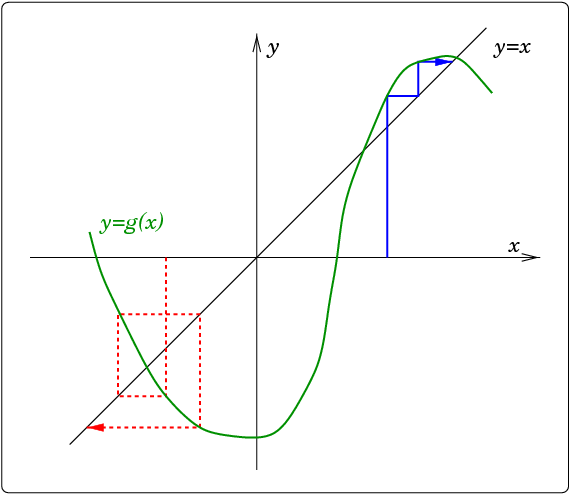
\includegraphics[width=0.95\textwidth]{figures/picard}
      \end{center}
    \end{column}
  \end{columns}

\end{frame}

\begin{frame}
  \frametitle{Geometric interpretations}

  \begin{columns}
    \begin{column}{0.5\textwidth}
      \begin{overlayarea}{\textwidth}{0.6\textheight}
        \only<1-4|handout:1>
        {
          \begin{itemize}
          \item<1-4> If $g$ does not intersect $y=x$, no fixed points (top left).
          \item<2-4> If range outside domain, sequence
            may not have a limit (top right).
          \item<3-4> If slope less than 1, function has a unique
            fixed point (bottom right).
          \end{itemize}
        }
        \only<4-|handout:1>
        {
          Not all fixed points \emph{stable} (top right, bottom left): no numerical implementation would converge.
        }
        % \only<4-|handout:2>
        % {
        %   Not all fixed points \emph{stable} (top right, bottom left): no numerical implementation would converge.

        %   Why are some intersections of $g$ and $y=x$ ``not fixed
        %   points'' (top right, bottom left)?
        % }
        % \only<5|handout:2>
        % {
        %   \vspace{2ex}

        %   Because the fixed point is not stable - no numerical
        %   implementation would converge.

        % }
      \end{overlayarea}
    \end{column}
    \begin{column}{0.5\textwidth}
      \begin{center}
        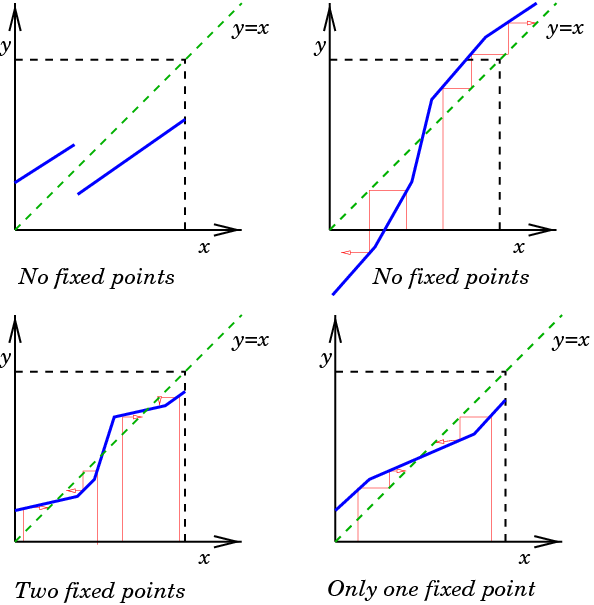
\includegraphics[width=0.95\textwidth]{figures/contract_examples}
      \end{center}
    \end{column}
  \end{columns}

\end{frame}

\begin{frame}
  \frametitle{Graphical examples - 1}

  \begin{columns}
    \begin{column}{0.475\textwidth}
      Let us try to find the root of
      \begin{equation*}
        f(x) = x - \cos(x)
      \end{equation*}
      in the interval $[0, 1]$. \pause The fixed point map is
      \begin{align*}
        g(x) & = x - f(x) \\
        & = \cos(x),
      \end{align*}
      which obeys
      \begin{enumerate}
      \item $g(I) \subseteq I$, and
      \item $|g'(x)| < 1$ within the interval.
      \end{enumerate}
    \end{column}
    \begin{column}{0.525\textwidth}
      \begin{center}
        \includegraphics<2->[width=\textwidth]{figures/cos_plotmap_final}
      \end{center}\pause
      The results of the iteration are
      \begin{align*}
        x_0 & = 0 &
        x_1 & = 1 \\
        x_2 & = 0.540302 &
        x_{10} & = 0.731404 \\
        x_{50} & = 0.739085 &
        x_{100} & = 0.739085.
      \end{align*}
    \end{column}
  \end{columns}

\end{frame}


\begin{frame}
  \frametitle{Graphical examples - 2}

  \begin{columns}
    \begin{column}{0.475\textwidth}
      Let us try to find the root of
      \begin{equation*}
        f(x) = x^3 - 13 x + 18
      \end{equation*}
      in the interval $[1, 2.05]$. \pause A map that works is
      \begin{equation*}
        g(x)  = \frac{x^3 + 18}{13}
      \end{equation*}
      which equals $x$ at roots of $f$ (check!) and obeys
      \begin{enumerate}
      \item $g(I) \subseteq I$, and
      \item $|g'(x)| < 1$ within the interval.
      \end{enumerate}
    \end{column}
    \begin{column}{0.525\textwidth}
      \begin{center}
        \includegraphics<2->[width=\textwidth]{figures/poly_plotmap_final}
      \end{center}\pause
      The results of the iteration are
      \begin{align*}
        x_0 & = 1 &
        x_1 & = 1.461538 \\
        x_2 & = 1.624768 &
        x_{10} & = 1.911737 \\
        x_{50} & = 1.997695 &
        x_{100} & = 1.999958.
      \end{align*}
    \end{column}
  \end{columns}

\end{frame}


\subsection{Contraction maps and theoretical results}

\begin{frame}
  \frametitle{From intuition to theory}

  Geometric intuition gives: a continuous iterative map, with the
  range within the domain, and slope less than 1, will have a unique
  fixed point. \pause To prove this need:

  \vspace{1ex}

  {\bf Definition}: A \emph{contracting map} is a continuous map
  $g(x) : [a, b] = I \subseteq \mathbb{R} \rightarrow \mathbb{R}$ if
  \begin{enumerate}
  \item $g(I) \subseteq I \Leftrightarrow g(x) \in I \, \, \, \forall
    x \in I$; \pause
  \item $g(x)$ is \emph{Lipschitz} continuous with constant $L < 1$:
    \begin{equation*}
      | g(x) - g(y) | \leq L | x - y | \, \, \, \forall x, y \in I.
    \end{equation*}
  \end{enumerate} \pause

  \vspace{1ex}

  It is key that
  \begin{equation*}
    \left| \oda{g}{x} \right| \leq L.
  \end{equation*}

\end{frame}

\begin{frame}
  \frametitle{Existence}

  First theorem shows that a fixed point of a contracting map
  exists:

  \vspace{1ex}

  {\bf Theorem 1}: If the function $g(x)$ is continuous in $I = [a,
  b]$ and $g(I) \subseteq I$, then $g(x)$ has at least one fixed point
  in $I$. \pause

  \vspace{1ex}

  Theorem is stronger than we need; no need of Lipschitz continuity. \pause

  \vspace{1ex}

  Proof: look for fixed points of $g$ in exactly
  the way that we look for roots of $f$. Construct function $F(x) =
  g(x) - x$, changes sign within $I$, and use continuity.  Intermediate value theorem shows there is a point $s$ where $F$ vanishes, implying $g(s) = s$ and a fixed point.

\end{frame}

\begin{frame}
  \frametitle{Uniqueness}

  {\bf Contraction mapping theorem}: If $g(x)$ is a contraction
  mapping in $I$ then there exists one and only one fixed point in
  $I$. \pause

  \vspace{3ex}

  The notes contain a proof of a weaker version of this theorem that
  requires differentiability. If $g$ is differentiable then the Mean
  Value theorem can be used.

\end{frame}

\begin{frame}
  \frametitle{Speed of convergence}

  A fixed point may exist, but how fast will the iterative method find
  it? \pause

  \vspace{1ex}

  {\bf Theorem}: If $g(x)$ is a contracting map in $I$ then, for
  arbitrary $x_0 \in I$ the sequence $x_{n+1} = g(x_n)$ converges to
  the unique fixed point $s$ and the error $e_n = x_n - s$ obeys
  \begin{equation*}
    |e_n| \leq \frac{L^n}{1 - L} |x_1 - x_0|.
  \end{equation*} \pause

  \vspace{1ex}

  Proof: bound error in terms of previous error, then bound initial error by first step. Bound on error and $L < 1$ gives convergence. \pause

  \vspace{1ex}

  Theorem shows convergence depends strongly on $L$, hence magnitude of derivative. Smaller derivative gives faster convergence.

\end{frame}

\begin{frame}
  \frametitle{Examples revisited}

  \begin{overlayarea}{\textwidth}{\textheight}
    \only<1|handout:1>
    {
      \begin{columns}
        \begin{column}{0.475\textwidth}
          We looked at
          \begin{equation*}
            g(x) = \cos(x)
          \end{equation*}
          in the interval $[0, 1]$. It is a contracting map, but
          \begin{align*}
            \max_{x \in I} |g'(x)| & = \sin(1) \\
            & = 0.84147.
          \end{align*}
          We should not expect fast convergence.
        \end{column}
        \begin{column}{0.525\textwidth}
          \begin{center}
            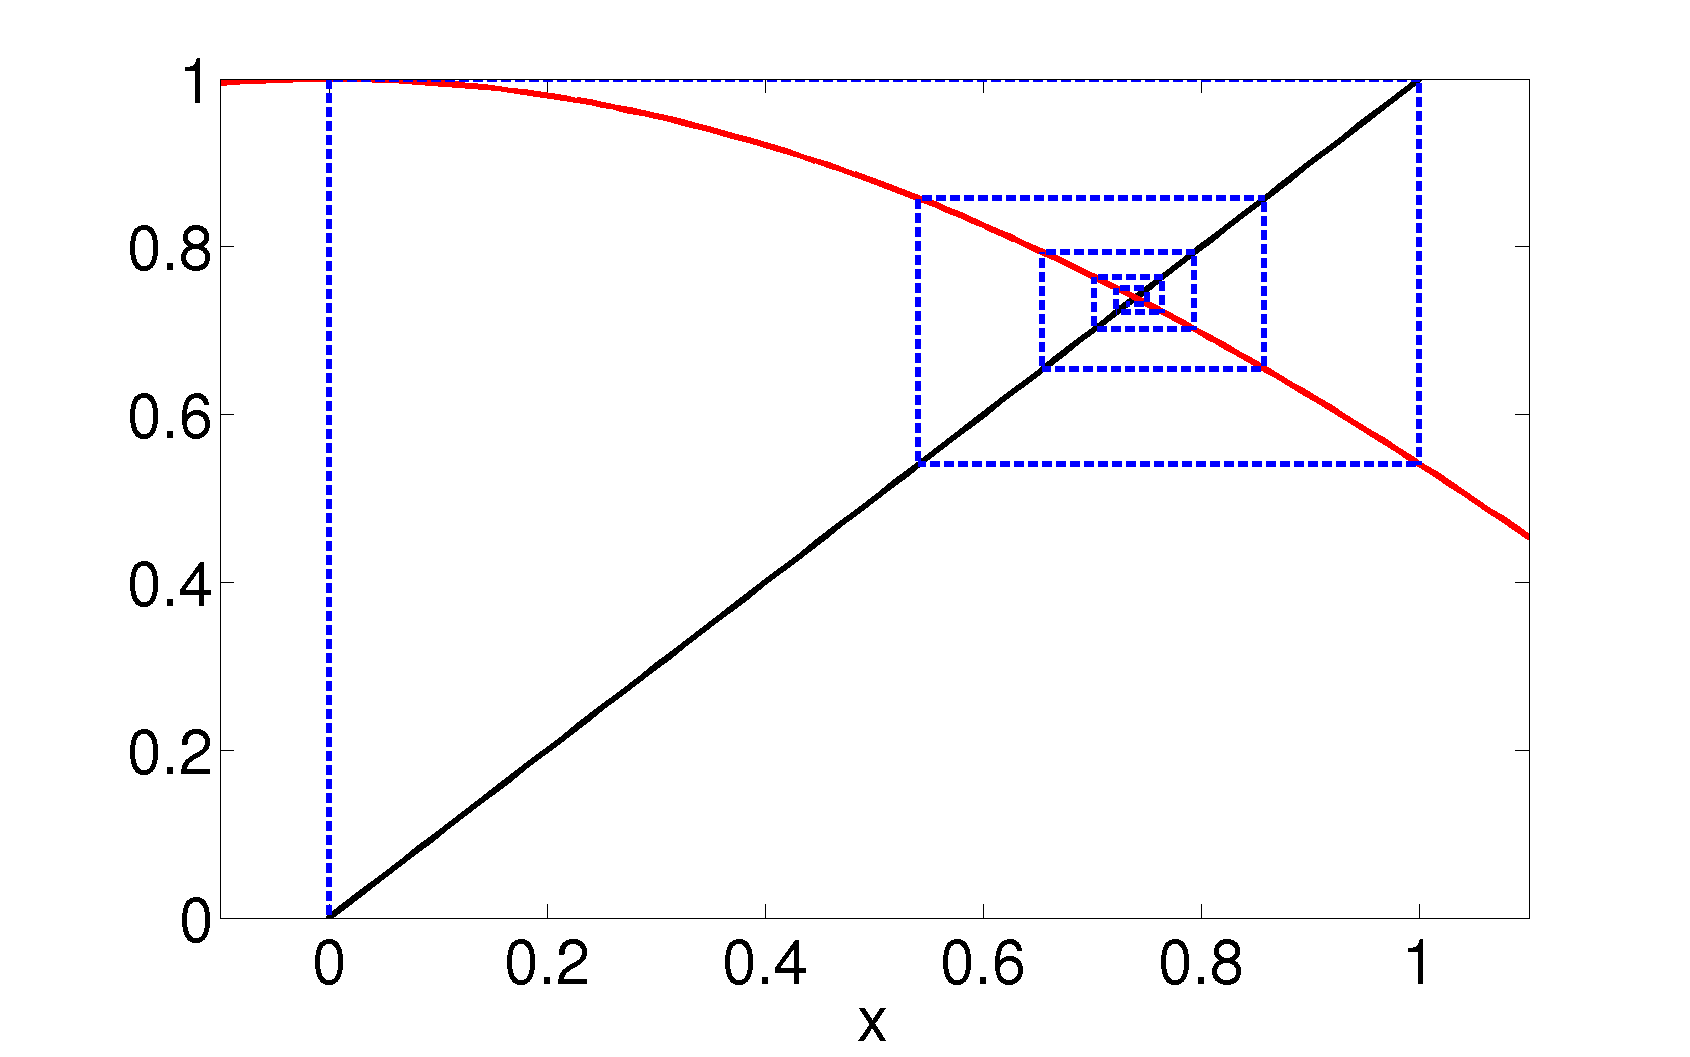
\includegraphics[width=\textwidth]{figures/cos_plotmap_final}
          \end{center}
          The results of the iteration are
          \begin{align*}
            x_0 & = 0 &
            x_1 & = 1 \\
            x_2 & = 0.540302 &
            x_{10} & = 0.731404 \\
            x_{50} & = 0.739085 &
            x_{100} & = 0.739085.
          \end{align*}
        \end{column}
      \end{columns}
    }
    \only<2|handout:2>
    {
  \begin{columns}
    \begin{column}{0.475\textwidth}
      We looked at
      \begin{equation*}
        g(x)  = \frac{x^3 + 18}{13}
      \end{equation*}
      in the interval $[1, 2.05]$. The map is monotonic and the
      largest value of the derivative is
      \begin{equation*}
        |g'(2.05)| = 0.97!
      \end{equation*}
      We therefore expect very slow convergence.
    \end{column}
    \begin{column}{0.525\textwidth}
      \begin{center}
        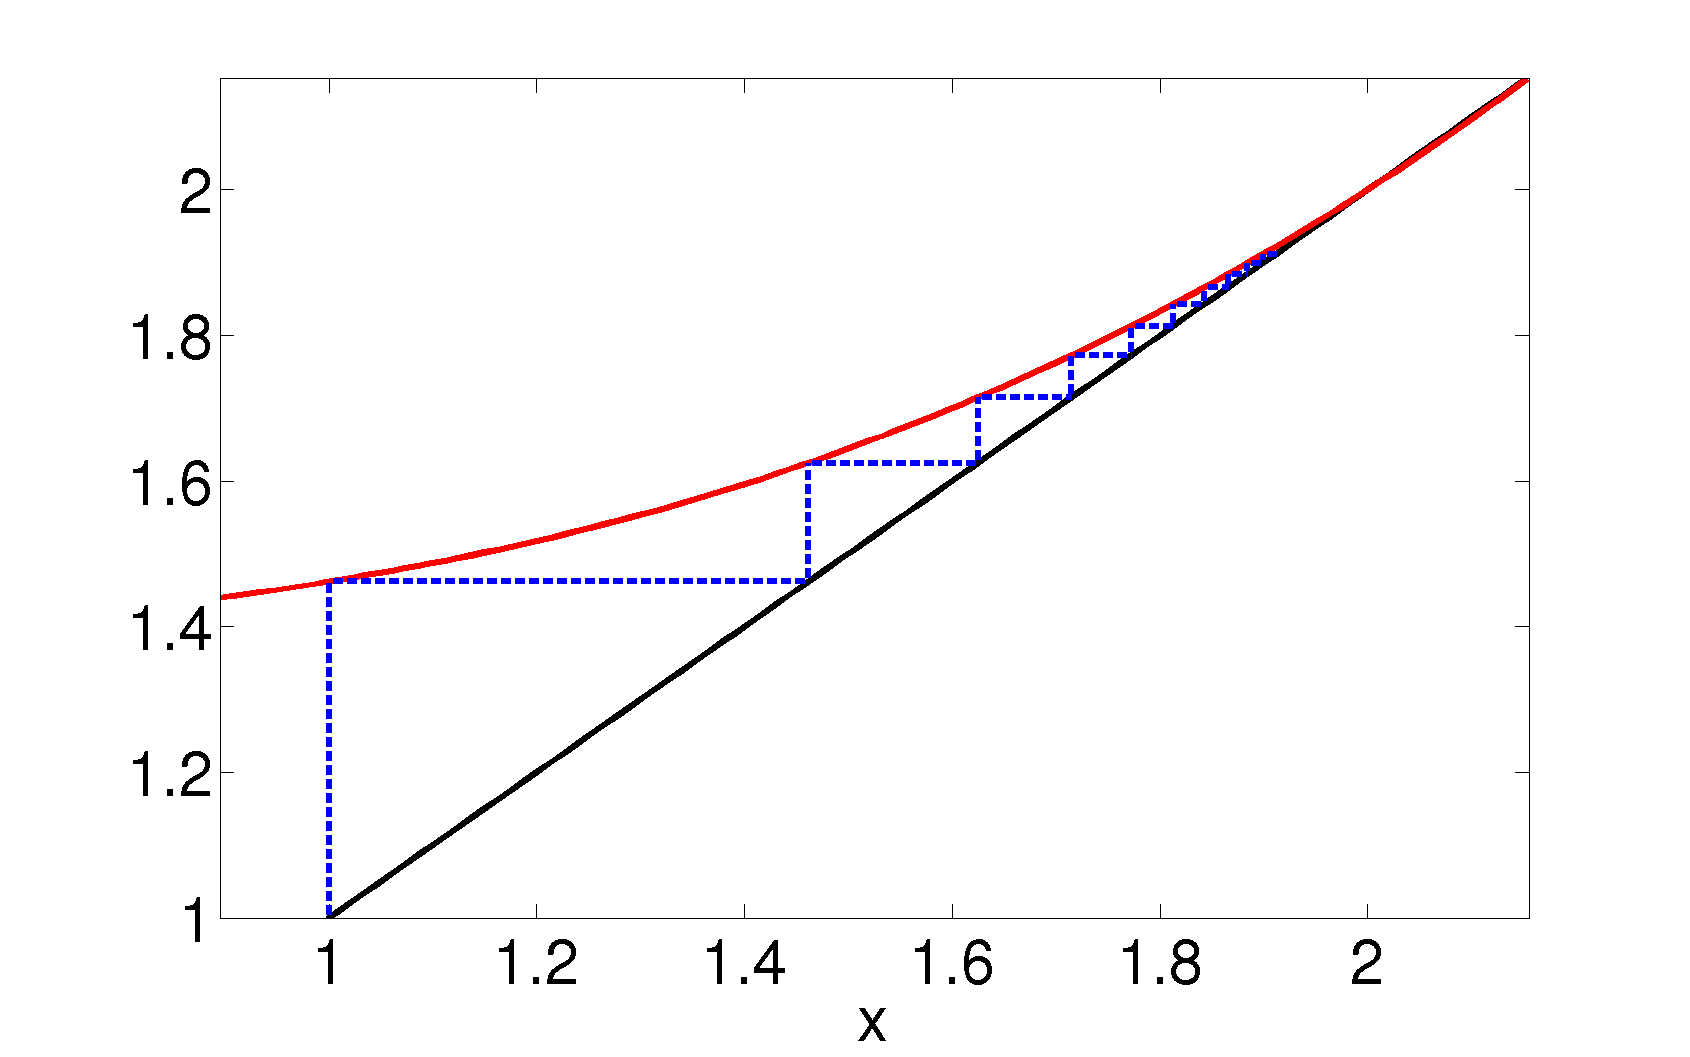
\includegraphics[width=\textwidth]{figures/poly_plotmap_final}
      \end{center}
      The results of the iteration are
      \begin{align*}
        x_0 & = 1 &
        x_1 & = 1.461538 \\
        x_2 & = 1.624768 &
        x_{10} & = 1.911737 \\
        x_{50} & = 1.997695 &
        x_{100} & = 1.999958.
      \end{align*}
    \end{column}
  \end{columns}
    }
  \end{overlayarea}

\end{frame}

\section{Summary}


\subsection{Summary}

\begin{frame}
  \frametitle{Summary}

  \begin{itemize}
  \item Fixed point or functional iteration methods for finding the
    root of $f(x)$ look for fixed points of
    \begin{equation*}
      g(x) = x - f(x).
    \end{equation*}
  \item Typically, the faster the scheme converges the closer the
    initial guess needs to be.
  \item Existence and uniqueness of the root found can be proved if
    $g$ is a contraction mapping for which
    \begin{enumerate}
    \item $g(I) \subseteq I$
    \item $g$ is Lipschitz continuous with $L < 1$.
    \end{enumerate}
  \item The speed of convergence is related to $L$ - the smaller $L$,
    the faster the convergence.
  \item {\bf All the results refer to the map $g$, not the original
      function $f$. $g$ can be chosen freely, provided the fixed point
      is a root of $f$!}
  \end{itemize}

\end{frame}

\section{Does it contract?}

\begin{frame}
\frametitle{Does it contract? Question 1}

\begin{columns}
    \begin{column}{0.45\textwidth}
  {\bf Definition}: A \emph{contracting map} is a continuous map
  $g(x) : [a, b] = I \subseteq \mathbb{R} \rightarrow \mathbb{R}$ if
\begin{enumerate}
  \item $g(I) \subseteq I \Leftrightarrow g(x) \in I \, \, \, \forall
    x \in I$;
  \item $g(x)$ is \emph{Lipschitz} continuous with constant $L < 1$:
    \begin{equation*}
      | g(x) - g(y) | \leq L | x - y | \, \, \, \forall x, y \in I.
    \end{equation*}
  \end{enumerate}
\end{column}
\begin{column}{0.55\textwidth}
  \begin{center}
   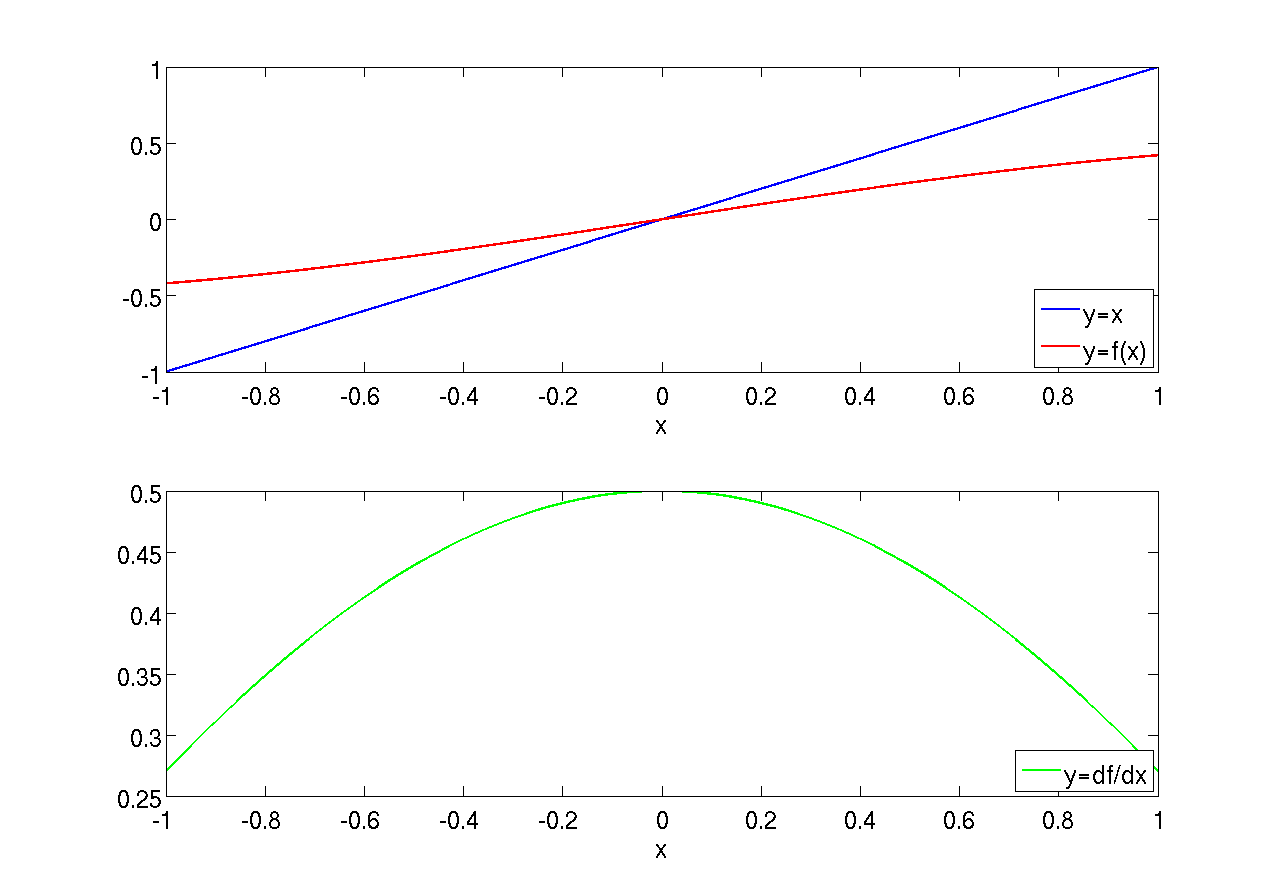
\includegraphics[width=\textwidth]{figures/cmap1}
  \end{center}
\end{column}
\end{columns}
\begin{overlayarea}{\textwidth}{0.1\textheight}
Does it contract?
\end{overlayarea}
\end{frame}

\begin{frame}
\frametitle{Does it contract? Question 2}

\begin{columns}
    \begin{column}{0.45\textwidth}
  {\bf Definition}: A \emph{contracting map} is a continuous map
  $g(x) : [a, b] = I \subseteq \mathbb{R} \rightarrow \mathbb{R}$ if
\begin{enumerate}
  \item $g(I) \subseteq I \Leftrightarrow g(x) \in I \, \, \, \forall
    x \in I$;
  \item $g(x)$ is \emph{Lipschitz} continuous with constant $L < 1$:
    \begin{equation*}
      | g(x) - g(y) | \leq L | x - y | \, \, \, \forall x, y \in I.
    \end{equation*}
  \end{enumerate}
\end{column}
\begin{column}{0.55\textwidth}
  \begin{center}
   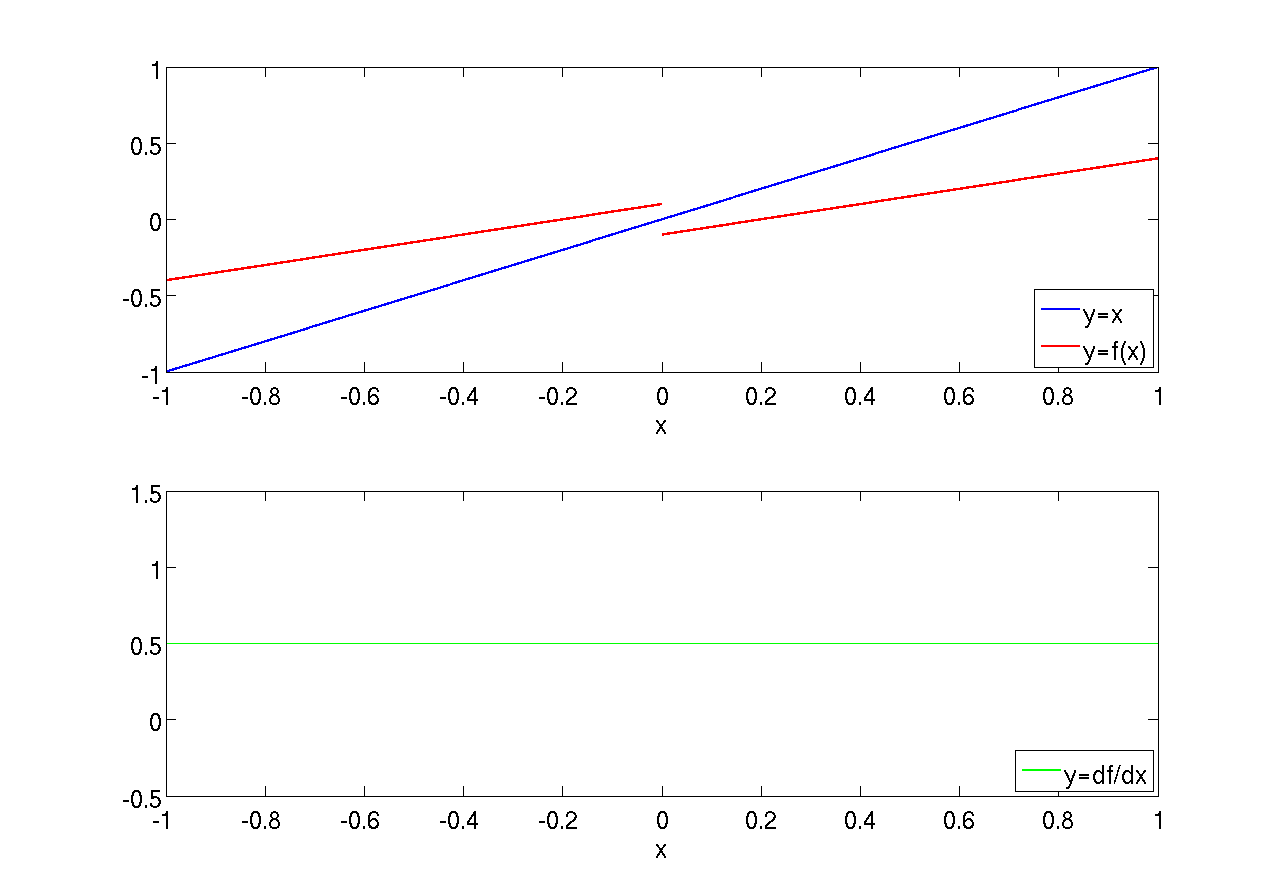
\includegraphics[width=\textwidth]{figures/cmap3}
  \end{center}
\end{column}
\end{columns}
\begin{overlayarea}{\textwidth}{0.1\textheight}
Does it contract?
\end{overlayarea}
\end{frame}

\begin{frame}
\frametitle{Does it contract? Question 3}

\begin{columns}
    \begin{column}{0.45\textwidth}
  {\bf Definition}: A \emph{contracting map} is a continuous map
  $g(x) : [a, b] = I \subseteq \mathbb{R} \rightarrow \mathbb{R}$ if
\begin{enumerate}
  \item $g(I) \subseteq I \Leftrightarrow g(x) \in I \, \, \, \forall
    x \in I$;
  \item $g(x)$ is \emph{Lipschitz} continuous with constant $L < 1$:
    \begin{equation*}
      | g(x) - g(y) | \leq L | x - y | \, \, \, \forall x, y \in I.
    \end{equation*}
  \end{enumerate}
\end{column}
\begin{column}{0.55\textwidth}
  \begin{center}
   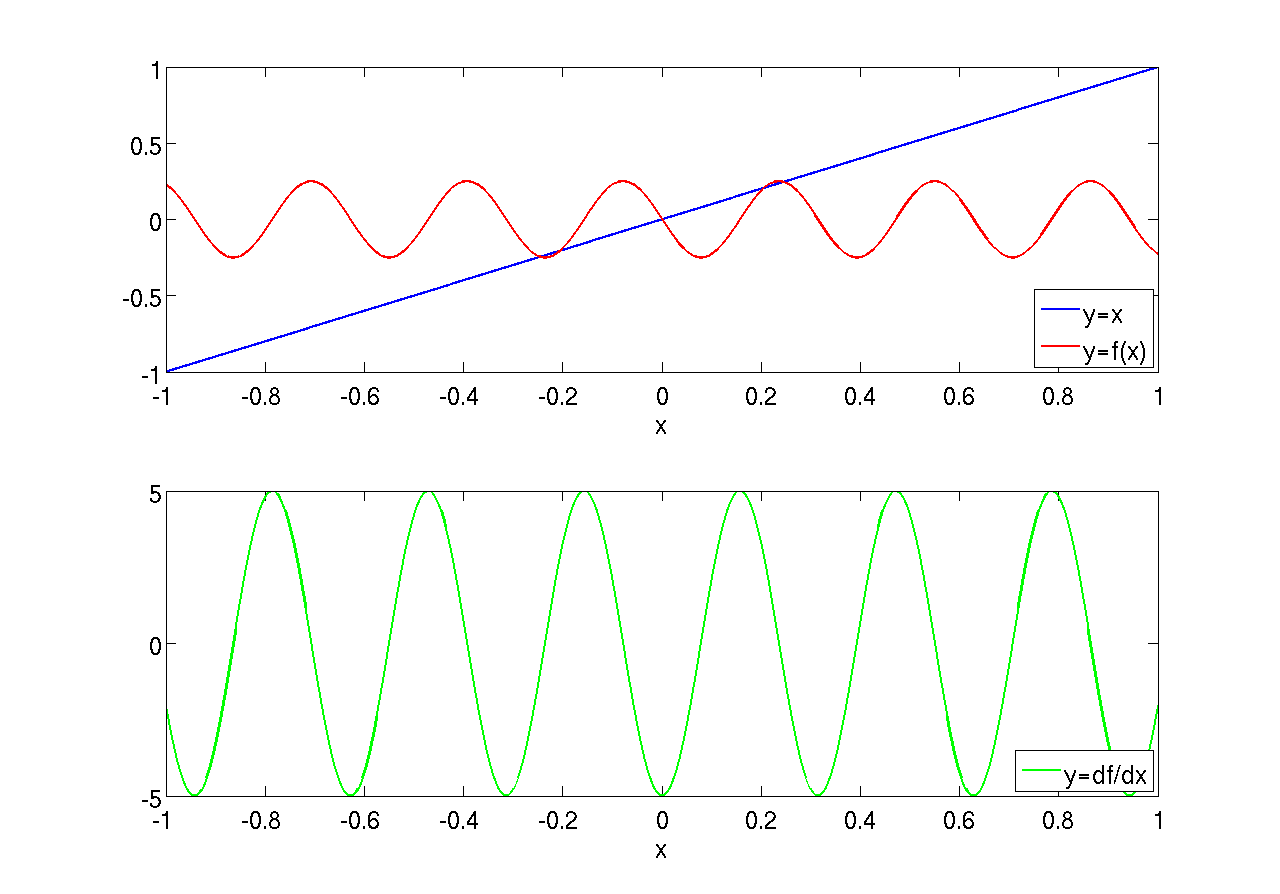
\includegraphics[width=\textwidth]{figures/cmap5}
  \end{center}
\end{column}
\end{columns}
\begin{overlayarea}{\textwidth}{0.1\textheight}
Does it contract?
\end{overlayarea}
\end{frame}

\begin{frame}
\frametitle{Does it contract? Question 4}

\begin{columns}
    \begin{column}{0.45\textwidth}
  {\bf Definition}: A \emph{contracting map} is a continuous map
  $g(x) : [a, b] = I \subseteq \mathbb{R} \rightarrow \mathbb{R}$ if
\begin{enumerate}
  \item $g(I) \subseteq I \Leftrightarrow g(x) \in I \, \, \, \forall
    x \in I$;
  \item $g(x)$ is \emph{Lipschitz} continuous with constant $L < 1$:
    \begin{equation*}
      | g(x) - g(y) | \leq L | x - y | \, \, \, \forall x, y \in I.
    \end{equation*}
  \end{enumerate}
\end{column}
\begin{column}{0.55\textwidth}
  \begin{center}
   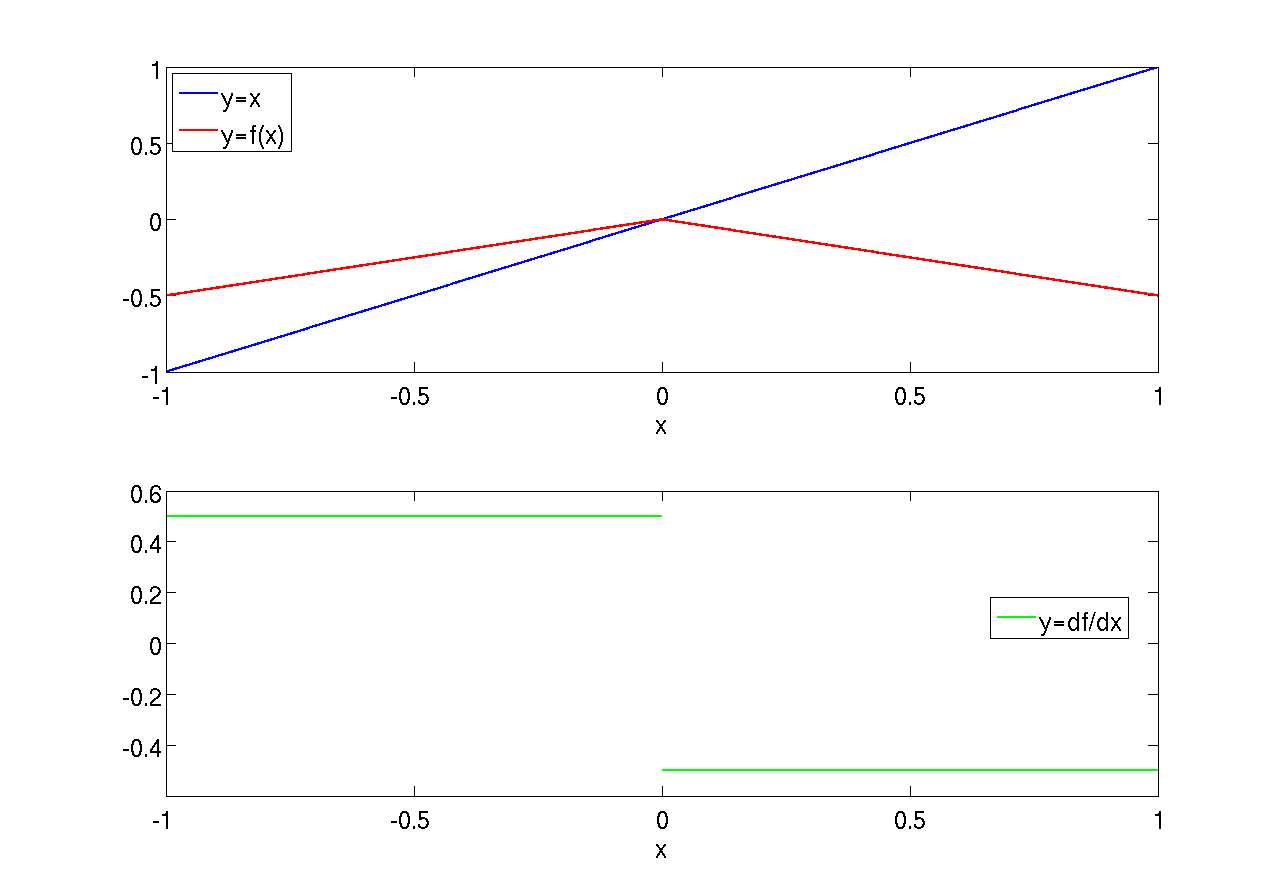
\includegraphics[width=\textwidth]{figures/cmap4}
  \end{center}
\end{column}
\end{columns}
\begin{overlayarea}{\textwidth}{0.1\textheight}
Does it contract?
\end{overlayarea}
\end{frame}

\begin{frame}
\frametitle{Does it contract? Question 5}

\begin{columns}
    \begin{column}{0.45\textwidth}
  {\bf Definition}: A \emph{contracting map} is a continuous map
  $g(x) : [a, b] = I \subseteq \mathbb{R} \rightarrow \mathbb{R}$ if
\begin{enumerate}
  \item $g(I) \subseteq I \Leftrightarrow g(x) \in I \, \, \, \forall
    x \in I$;
  \item $g(x)$ is \emph{Lipschitz} continuous with constant $L < 1$:
    \begin{equation*}
      | g(x) - g(y) | \leq L | x - y | \, \, \, \forall x, y \in I.
    \end{equation*}
  \end{enumerate}
\end{column}
\begin{column}{0.55\textwidth}
  \begin{center}
   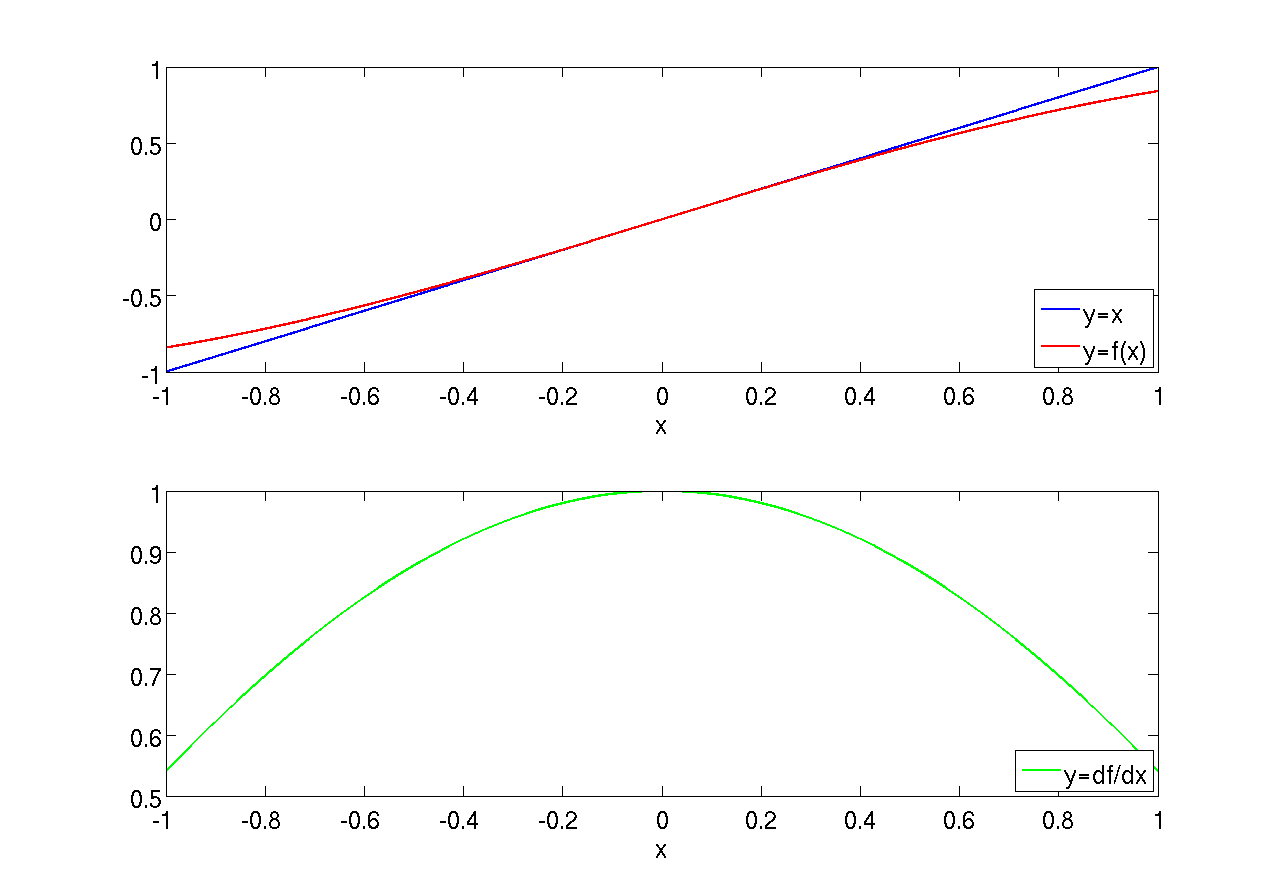
\includegraphics[width=\textwidth]{figures/cmap2}
  \end{center}
\end{column}
\end{columns}
\begin{overlayarea}{\textwidth}{0.1\textheight}
Does it contract?
\end{overlayarea}
\end{frame}

\begin{frame}
\frametitle{Does it contract? Question 6}

\begin{columns}
    \begin{column}{0.45\textwidth}
  {\bf Definition}: A \emph{contracting map} is a continuous map
  $g(x) : [a, b] = I \subseteq \mathbb{R} \rightarrow \mathbb{R}$ if
\begin{enumerate}
  \item $g(I) \subseteq I \Leftrightarrow g(x) \in I \, \, \, \forall
    x \in I$;
  \item $g(x)$ is \emph{Lipschitz} continuous with constant $L < 1$:
    \begin{equation*}
      | g(x) - g(y) | \leq L | x - y | \, \, \, \forall x, y \in I.
    \end{equation*}
  \end{enumerate}
\end{column}
\begin{column}{0.55\textwidth}
  \begin{center}
   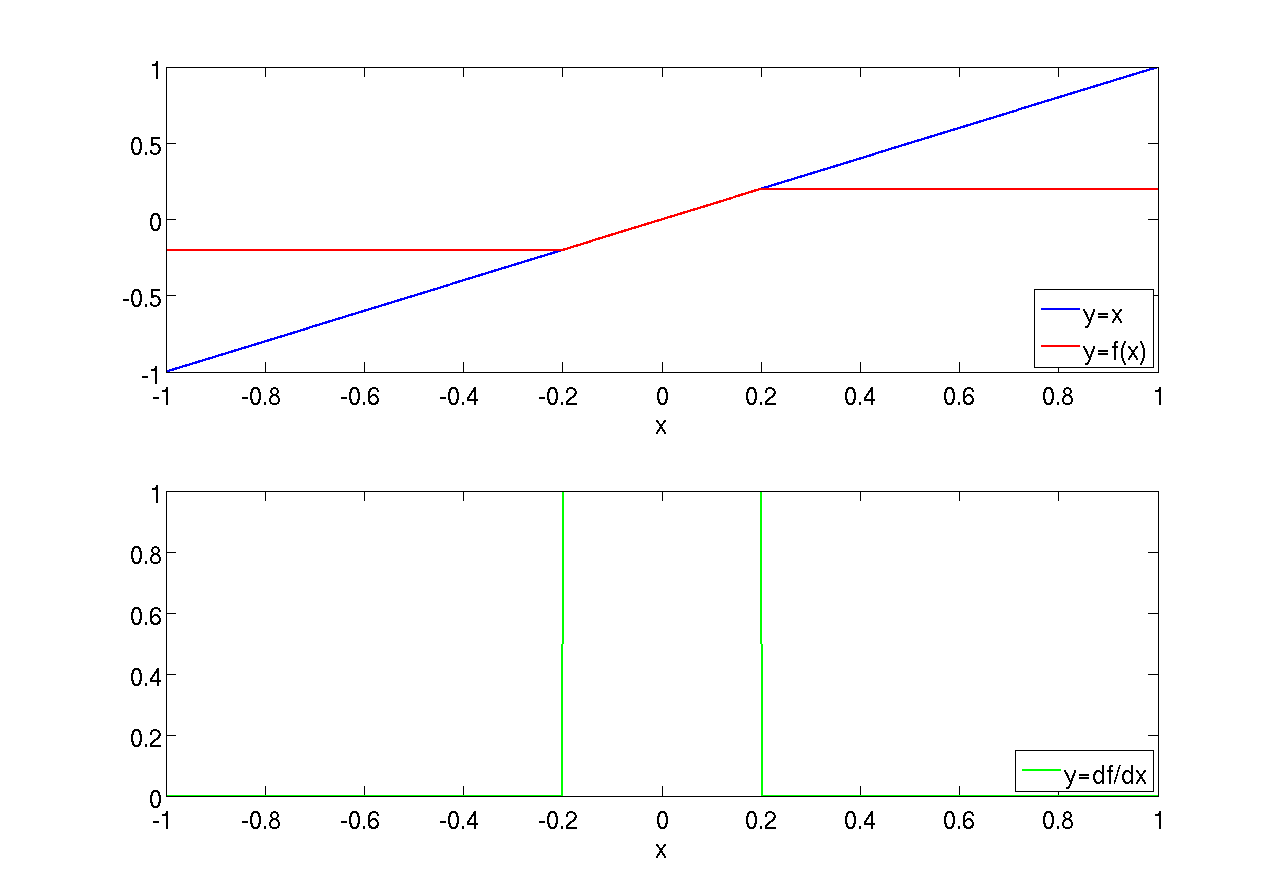
\includegraphics[width=\textwidth]{figures/cmap9}
  \end{center}
\end{column}
\end{columns}
\begin{overlayarea}{\textwidth}{0.1\textheight}
Does it contract?
\end{overlayarea}
\end{frame}

\begin{frame}
\frametitle{Does it contract? Answer 1}

\begin{columns}
    \begin{column}{0.45\textwidth}
  {\bf Definition}: A \emph{contracting map} is a continuous map
  $g(x) : [a, b] = I \subseteq \mathbb{R} \rightarrow \mathbb{R}$ if
\begin{enumerate}
  \item $g(I) \subseteq I \Leftrightarrow g(x) \in I \, \, \, \forall
    x \in I$;
  \item $g(x)$ is \emph{Lipschitz} continuous with constant $L < 1$:
    \begin{equation*}
      | g(x) - g(y) | \leq L | x - y | \, \, \, \forall x, y \in I.
    \end{equation*}
  \end{enumerate}
\end{column}
\begin{column}{0.55\textwidth}
  \begin{center}
   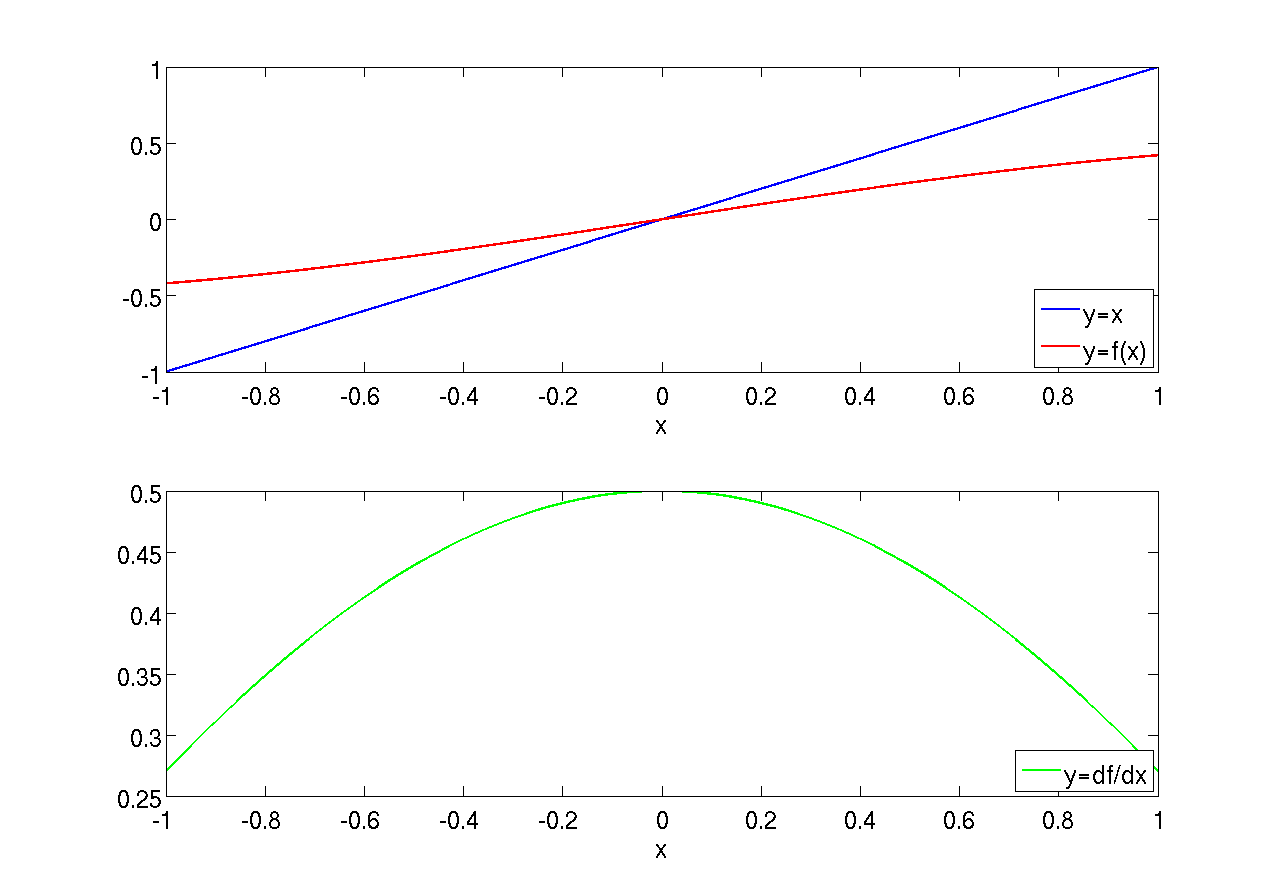
\includegraphics[width=\textwidth]{figures/cmap1}
  \end{center}
\end{column}
\end{columns}
\begin{overlayarea}{\textwidth}{0.1\textheight}
Does it contract?  \only<2->{Yes! Both the conditions are met.}
\end{overlayarea}
\end{frame}

\begin{frame}
\frametitle{Does it contract? Answer 2}

\begin{columns}
    \begin{column}{0.45\textwidth}
  {\bf Definition}: A \emph{contracting map} is a continuous map
  $g(x) : [a, b] = I \subseteq \mathbb{R} \rightarrow \mathbb{R}$ if
\begin{enumerate}
  \item $g(I) \subseteq I \Leftrightarrow g(x) \in I \, \, \, \forall
    x \in I$;
  \item $g(x)$ is \emph{Lipschitz} continuous with constant $L < 1$:
    \begin{equation*}
      | g(x) - g(y) | \leq L | x - y | \, \, \, \forall x, y \in I.
    \end{equation*}
  \end{enumerate}
\end{column}
\begin{column}{0.55\textwidth}
  \begin{center}
   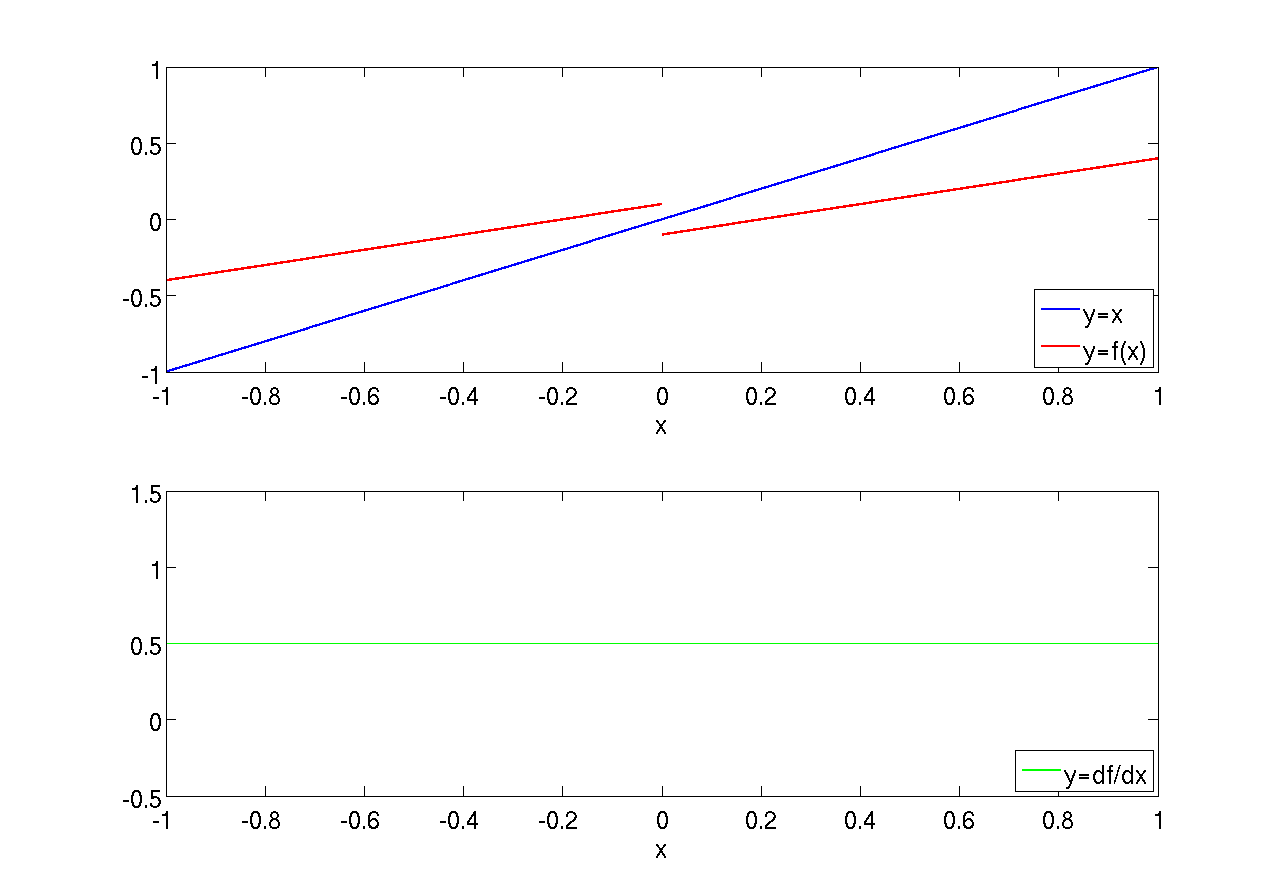
\includegraphics[width=\textwidth]{figures/cmap3}
  \end{center}
\end{column}
\end{columns}
\begin{overlayarea}{\textwidth}{0.1\textheight}
Does it contract?  \only<2->{No! There are no fixed points of the map.  The continuity condition has failed.}
\end{overlayarea}
\end{frame}

\begin{frame}
\frametitle{Does it contract? Answer 3}

\begin{columns}
    \begin{column}{0.45\textwidth}
  {\bf Definition}: A \emph{contracting map} is a continuous map
  $g(x) : [a, b] = I \subseteq \mathbb{R} \rightarrow \mathbb{R}$ if
\begin{enumerate}
  \item $g(I) \subseteq I \Leftrightarrow g(x) \in I \, \, \, \forall
    x \in I$;
  \item $g(x)$ is \emph{Lipschitz} continuous with constant $L < 1$:
    \begin{equation*}
      | g(x) - g(y) | \leq L | x - y | \, \, \, \forall x, y \in I.
    \end{equation*}
  \end{enumerate}
\end{column}
\begin{column}{0.55\textwidth}
  \begin{center}
   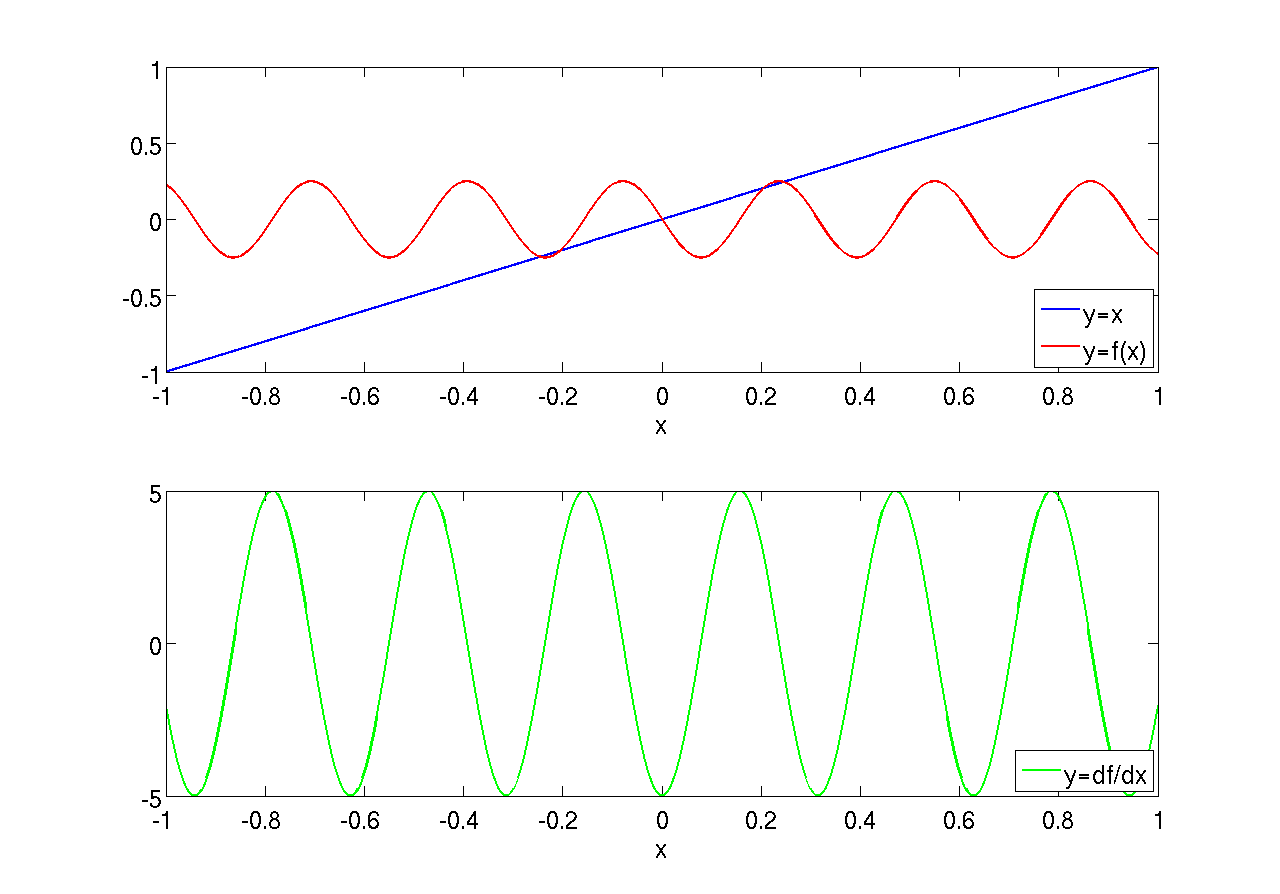
\includegraphics[width=\textwidth]{figures/cmap5}
  \end{center}
\end{column}
\end{columns}
\begin{overlayarea}{\textwidth}{0.1\textheight}
Does it contract?  \only<2->{No! Although the function is contained in its interval the second condition is not met.}
\end{overlayarea}
\end{frame}

\begin{frame}
\frametitle{Does it contract? Answer 4}

\begin{columns}
    \begin{column}{0.45\textwidth}
  {\bf Definition}: A \emph{contracting map} is a continuous map
  $g(x) : [a, b] = I \subseteq \mathbb{R} \rightarrow \mathbb{R}$ if
\begin{enumerate}
  \item $g(I) \subseteq I \Leftrightarrow g(x) \in I \, \, \, \forall
    x \in I$;
  \item $g(x)$ is \emph{Lipschitz} continuous with constant $L < 1$:
    \begin{equation*}
      | g(x) - g(y) | \leq L | x - y | \, \, \, \forall x, y \in I.
    \end{equation*}
  \end{enumerate}
\end{column}
\begin{column}{0.55\textwidth}
  \begin{center}
   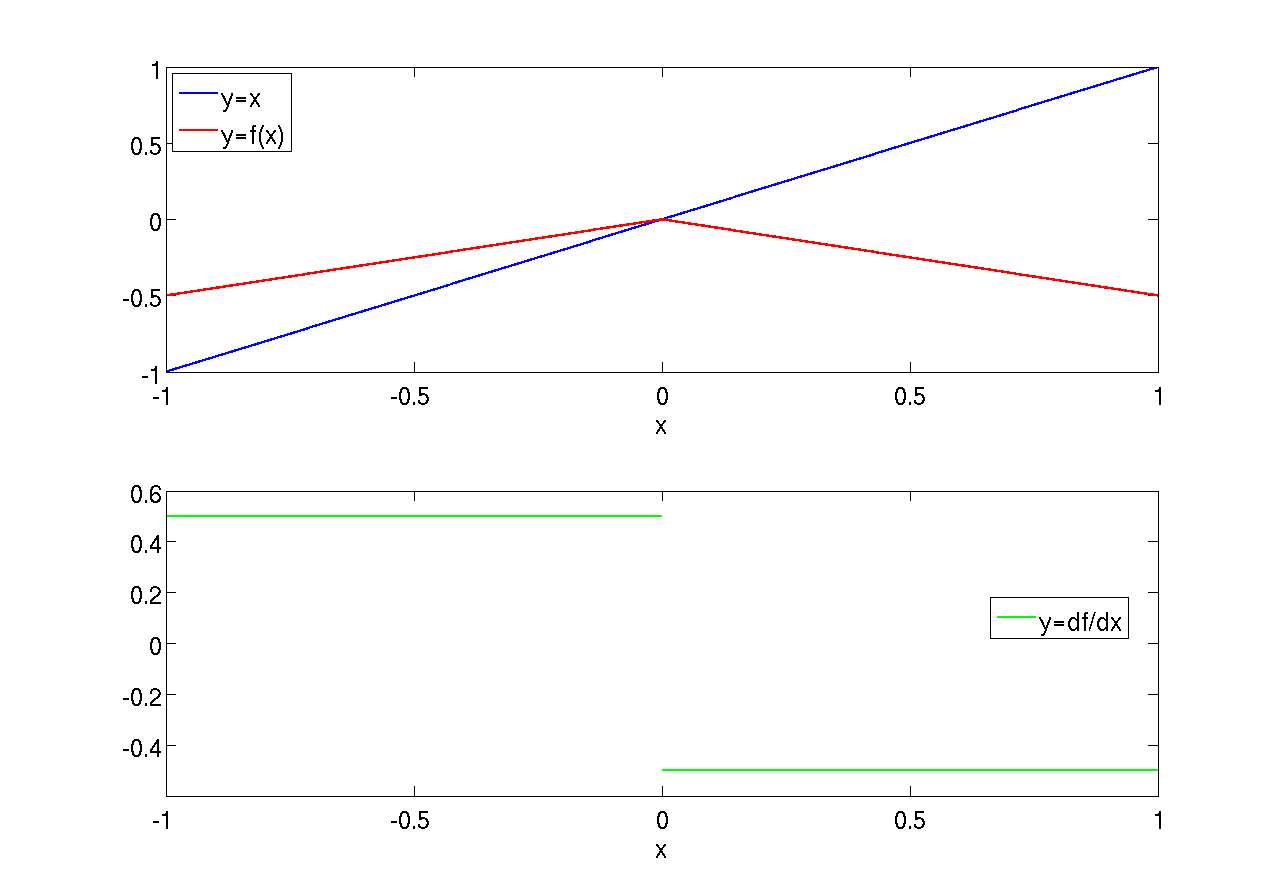
\includegraphics[width=\textwidth]{figures/cmap4}
  \end{center}
\end{column}
\end{columns}
\begin{overlayarea}{\textwidth}{0.1\textheight}
Does it contract?  \only<2->{Yes! Even though there is a jump in the derivative both conditions are met.}
\end{overlayarea}
\end{frame}

\begin{frame}
\frametitle{Does it contract? Answer 5}

\begin{columns}
    \begin{column}{0.45\textwidth}
  {\bf Definition}: A \emph{contracting map} is a continuous map
  $g(x) : [a, b] = I \subseteq \mathbb{R} \rightarrow \mathbb{R}$ if
\begin{enumerate}
  \item $g(I) \subseteq I \Leftrightarrow g(x) \in I \, \, \, \forall
    x \in I$;
  \item $g(x)$ is \emph{Lipschitz} continuous with constant $L < 1$:
    \begin{equation*}
      | g(x) - g(y) | \leq L | x - y | \, \, \, \forall x, y \in I.
    \end{equation*}
  \end{enumerate}
\end{column}
\begin{column}{0.55\textwidth}
  \begin{center}
   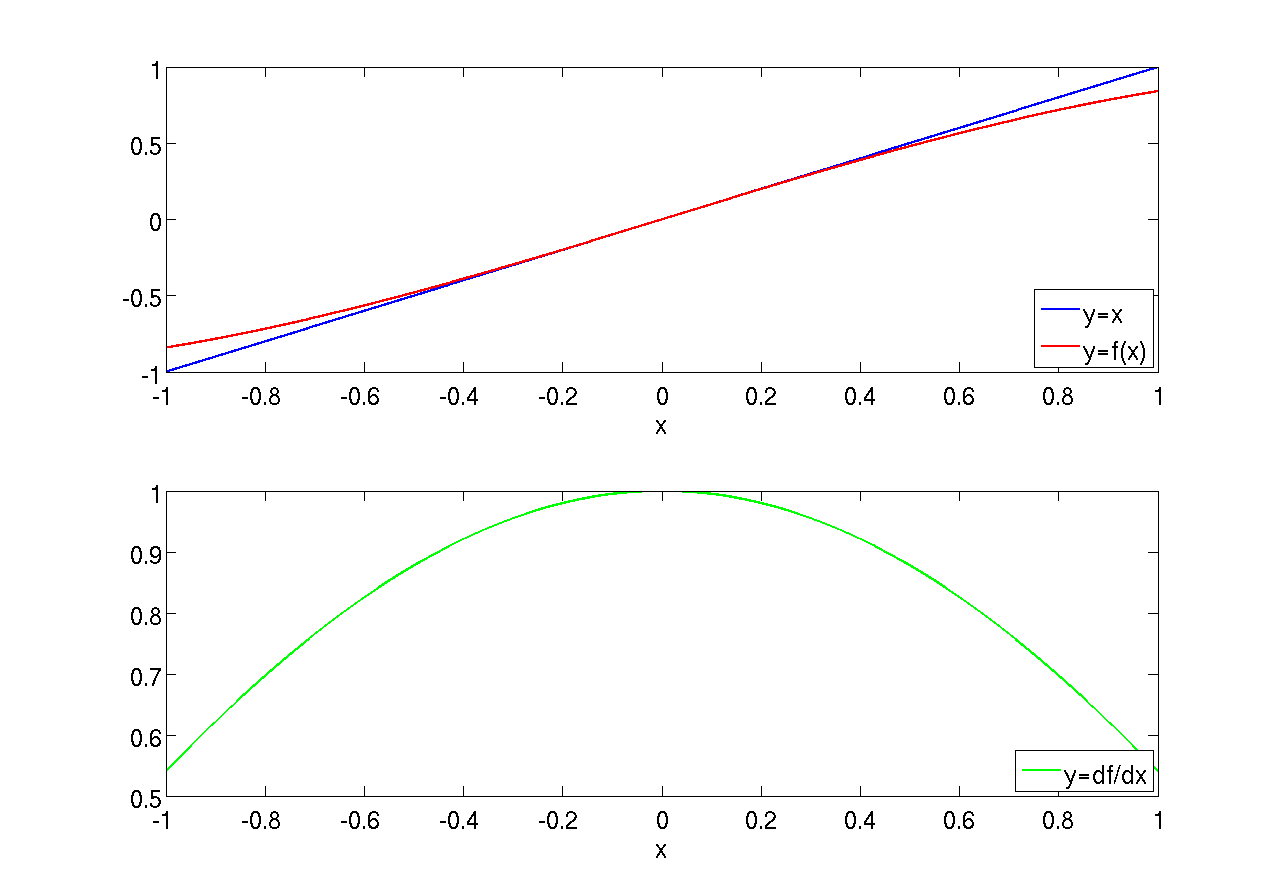
\includegraphics[width=\textwidth]{figures/cmap2}
  \end{center}
\end{column}
\end{columns}
\begin{overlayarea}{\textwidth}{0.1\textheight}
Does it contract?  \only<2->{No! The derivative is 1 and we cannot guarantee that there is only one fixed point.}
\end{overlayarea}
\end{frame}

\begin{frame}
\frametitle{Does it contract? Answer 6}

\begin{columns}
    \begin{column}{0.45\textwidth}
  {\bf Definition}: A \emph{contracting map} is a continuous map
  $g(x) : [a, b] = I \subseteq \mathbb{R} \rightarrow \mathbb{R}$ if
\begin{enumerate}
  \item $g(I) \subseteq I \Leftrightarrow g(x) \in I \, \, \, \forall
    x \in I$;
  \item $g(x)$ is \emph{Lipschitz} continuous with constant $L < 1$:
    \begin{equation*}
      | g(x) - g(y) | \leq L | x - y | \, \, \, \forall x, y \in I.
    \end{equation*}
  \end{enumerate}
\end{column}
\begin{column}{0.55\textwidth}
  \begin{center}
   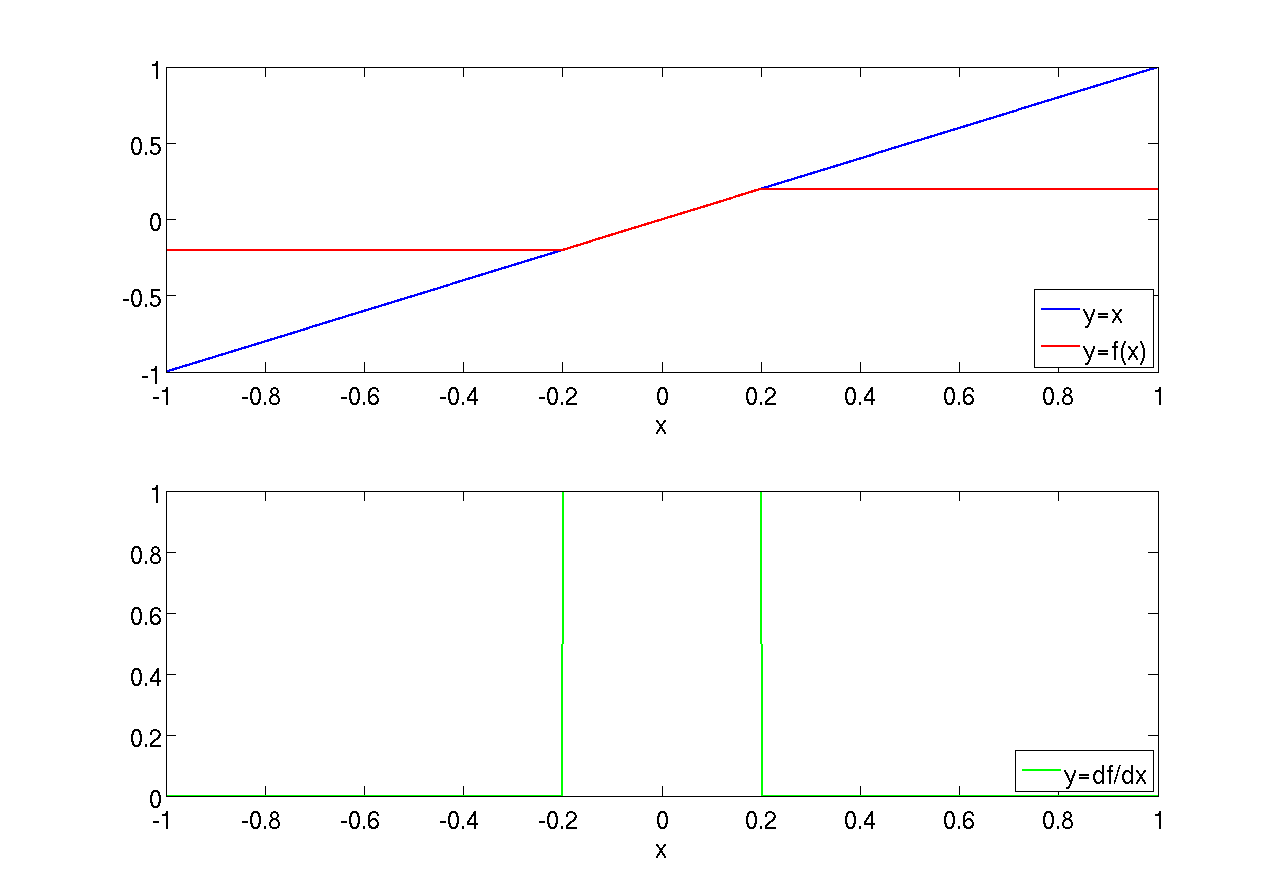
\includegraphics[width=\textwidth]{figures/cmap9}
  \end{center}
\end{column}
\end{columns}
\begin{overlayarea}{\textwidth}{0.1\textheight}
Does it contract?  \only<2->{No! The derivative is 1 and we cannot guarantee that there is only one fixed point.  In this case there is a whole line of fixed points.}
\end{overlayarea}
\end{frame}

\end{document}



%%% Local Variables:
%%% mode: latex
%%% TeX-master: t
%%% End:
